\section{Método: Corroboração entre Camadas}\label{sec:method}
Seja $\Delta_i=\theta_i-\theta_{\text{servidor}}$ a atualização achatada do cliente $i$,
fatiada por tensor de parâmetros $g$. Removemos o consenso centrando na mediana por coordenada,
$C_i=\Delta_i-\mathrm{median}_j(\Delta_j)$. Por tensor $g$, dois sinais descrevem o cliente $i$
em relação aos demais --- direção e norma:
\begin{equation}
s_g(i)=\max_{j\neq i}\cos\!\big(C_i[g],C_j[g]\big),\qquad n_g(i)=\lVert C_i[g]\rVert .
\end{equation}
Cada um é padronizado por um $z$ \emph{robusto} (mediana / MAD) entre os clientes, e o escore por
tensor sinaliza o cliente $i$ quando
\begin{equation}
z_g(i)=\max(z_{\text{sim}},0)+\max(z_{\text{norm}},0) > z_{\text{thr}}\;(=3).
\end{equation}

\textbf{Diagnóstico (vazamento convolucional).} Um agregador-sombra que apenas registra o sinal
(sem agir) mostra que, contra o LaySelFL, o atacante é sinalizado em $\approx 21$ tensores por
rodada (mediana; $p_{10}\approx12$), enquanto um cliente benigno é sinalizado em $\approx 1$
($p_{90}\approx7$) --- Fig.~\ref{fig:corrob}. O envenenamento está espalhado de forma rala por
muitos tensores convolucionais, de modo que decidir tensor a tensor descarta a evidência entre
tensores; é exatamente essa evidência agregada que separa os grupos.

\begin{figure}[t]\centering
  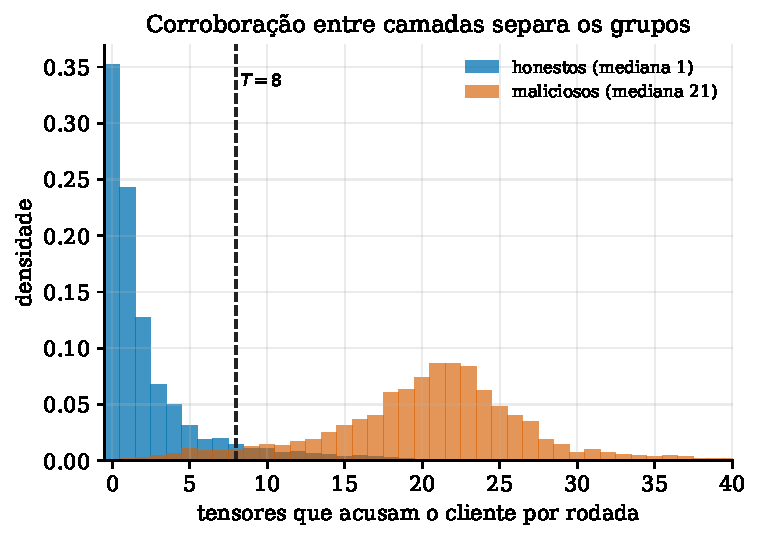
\includegraphics[width=\linewidth]{fig_corroboracao.pdf}
  \caption{Agregador-sombra no cenário fiel (4 sementes, rodadas de ataque 80--200): número de
  tensores que acusam cada cliente por rodada. Honestos concentram-se em $\approx 1$; maliciosos,
  em $\approx 21$. A decisão tensor a tensor joga fora essa separação.}
  \label{fig:corrob}
\end{figure}

\textbf{Corroboração.} Por isso \emph{contamos} os tensores que acusam e decidimos pelo cliente:
\begin{equation}
\text{contagem}_i=\sum_g [\,z_g(i)>z_{\text{thr}}\,],\qquad \text{confirmado se } \text{contagem}_i\geq T .
\end{equation}
A curva de detecção sobre $T$ (Fig.~\ref{fig:curvaT}) dá $F_1=0{,}88$ em $T{=}8$ (revocação
$0{,}95$, precisão $0{,}82$), com pico em $F_1=0{,}90$ ($T{=}12$). \textbf{A resposta} é modular:
remover o cliente confirmado de todos os tensores (\emph{corr}); expurgar completamente qualquer
cliente sinalizado (\emph{client}); ou substituir a contribuição suspeita pela mediana benigna,
preservando a massa de votos (\emph{corr-soft}).

\begin{figure}[t]\centering
  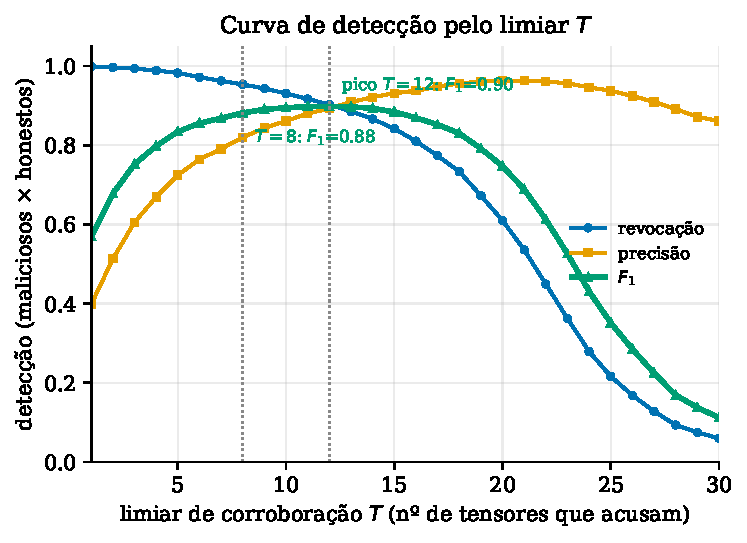
\includegraphics[width=0.92\linewidth]{fig_curva_T.pdf}
  \caption{Detecção de clientes maliciosos pelo limiar de corroboração $T$ (média de 4 sementes).
  Um patamar largo de $F_1$ alto ($T\in[6,16]$) torna a escolha de $T$ pouco sensível.}
  \label{fig:curvaT}
\end{figure}
